% Template for PLoS
% Version 1.0 January 2009
%
% To compile to PDF, run:
% latex plos.template
% bibtex plos.template
% latex plos.template
% latex plos.template
% dvipdf plos.template

% DO NOT EDIT - PLoS STYLE
\documentclass[10pt]{article}

% amsmath package, useful for mathematical formulas
\usepackage{amsmath}
% amssymb package, useful for mathematical symbols
\usepackage{amssymb}

% graphicx package, useful for including eps and pdf graphics
% include graphics with the command \includegraphics
\usepackage{graphicx}

% cite package, to clean up citations in the main text. Do not remove.
\usepackage{cite}

\usepackage{color} 
\usepackage{url}

% Use doublespacing - comment out for single spacing
\usepackage{setspace} 
\doublespacing

% Text layout
\topmargin 0.0cm
\oddsidemargin 0.5cm
\evensidemargin 0.5cm
\textwidth 16cm 
\textheight 21cm

% Bold the 'Figure #' in the caption and separate it with a period
% Captions will be left justified
\usepackage[labelfont=bf,labelsep=period,justification=raggedright]{caption}

% Use the PLoS provided bibtex style
\bibliographystyle{plos2009}

% Remove brackets from numbering in List of References
\makeatletter
\renewcommand{\@biblabel}[1]{\quad#1.}
\makeatother

% Leave date blank
\date{}

\pagestyle{myheadings}
%% ** EDIT HERE **

%% ** EDIT HERE **
%% PLEASE INCLUDE ALL MACROS BELOW
\newcommand{\highlight}[1]{{\color{red} \bf{#1}}}
\newcommand{\garycomment}[1]{{\color{green} \bf{Gary: #1}}}
\newcommand{\comment}[1]{{\color{green} \bf{#1}}}
%% END MACROS SECTION

% Article Structure
%    Title which includes the name of the software.
%    Authors and affiliations.
%    Abstract – Fundamental task(s) which the software accomplishes, examples of biological insights from the use of the software, details of availability, including where to download the most recent source code, the license, any operating system dependencies, and support mailing lists.
%    Introduction – A description of the problem addressed by the software and of its novelty and exceptional nature in addressing that problem.
%    Design and Implementation – Details of the algorithms used by the software, how those algorithms have been instantiated, including dependencies. Details of the supplied test data and how to install and run the software should be detailed in the supplementary material.
%    Results – Examples of biological problems solved using the software, including results obtained with the deposited test data and associated parameters.
%    Availability and Future Directions – Where the software has been deposited. Any future work planned to be carried out by the authors, how others might extend the software.
\begin{document}

% Title must be 150 characters or less
\begin{flushleft}
{\Large
\textbf{Chaste: an open source C++ library for computational physiology and biology}
}
% Insert Author names, affiliations and corresponding author email.
\\
Gary R. Mirams$^{1,\ast}$, Christopher J. Arthurs$^{1}$, Miguel O. Bernabeu$^{2}$, 
Rafael Bordas$^{1}$, Jonathan Cooper$^{1}$, Alberto Corrias$^3$, Yohan Davit$^4$, 
Sara-Jane Dunn$^5$, Alexander G. Fletcher$^6$, Daniel G. Harvey$^{1}$, 
James M. Osborne$^{1}$, Pras Pathmanathan$^{1,7}$, Joe M. Pitt-Francis$^{1}$, 
James Southern$^8$, Nejib Zemzemi$^9$, David J. Gavaghan$^{1}$
\\
\bf{1} Computational Biology, Department of Computer Science, University of Oxford, Oxford, UK
\\
\bf{2} CoMPLEX, Faculty of Maths \& Physical Sciences, University College London, London, UK
\\
\bf{3} Department of Bioengineering, National University of Singapore, Singapore, Singapore
\\
\bf{4} Oxford Centre for Collaborative Applied Mathematics, Mathematical Institute, University of Oxford, Oxford, UK
\\
\bf{5} Computational Science Laboratory, Microsoft Research, Cambridge, UK
\\
\bf{6} Centre for Mathematical Biology, Mathematical Institute, University of Oxford, Oxford, UK
\\
\bf{7} Food and Drug Administration, Silver Spring, Maryland, USA
\\
\bf{8} Fujitsu Laboratories of Europe, Hayes Park, London, UK
\\
\bf{9} INRIA, Bordeaux, France
\\
$\ast$ E-mail: \texttt{gary.mirams@cs.ox.ac.uk}
\end{flushleft}

% Please keep the abstract between 250 and 300 words
\section*{Abstract}
% PLoS Instructions:
% Fundamental task(s) which the software accomplishes, examples of biological insights from the use of the software, 
% details of availability, including where to download the most recent source code, the license, any operating system dependencies, and support mailing lists.
Chaste --- \textbf{C}ancer, \textbf{H}eart \textbf{A}nd \textbf{S}oft \textbf{T}issue \textbf{E}nvironment --- 
is an open source C++ library for the computational simulation of mathematical models developed for physiology and biology.
Code development has been driven by two initial applications: cardiac electrophysiology and cancer development. 
In cardiac electrophysiology a large number of studies have been enabled and performed, including high-performance computational investigations of defibrillation on realistic human cardiac geometry. 
New models for the initiation and growth of tumours have been developed.
In particular, individual-cell-based simulations have provided novel insight into the role of stem cells in the colorectal crypt.
Chaste is in constant evolution and is now being applied to a far wider range of problems. 
The code provides modules for handling common components of numerical analysis, such as meshes and solvers of ordinary and partial differential equations (ODEs/PDEs).
Re-use of these components avoids the need for researchers to `re-invent the wheel' with each new project, accelerating the rate of progress in new applications.
Chaste is developed using industrial techniques, in particular test-driven development, to ensure reliability.
The source code, both for releases and the development version, is available under an open source BSD licence to download at \texttt{http://www.cs.ox.ac.uk/chaste}, 
together with details of a mailing list and links to documentation and tutorials.
% Please keep the Author Summary between 150 and 200 words
% Use first person. 
\section*{Author Summary}
% Lay-person summary 

It is often the case that scientific software is written for a specific purpose, by a single researcher. 
Moreover, such code can be discarded after it has served its purpose, or inherited by a new user who is forced to translate the style, purpose and possible errors encoded by the original developer, which can delay new progress. 
To move away from this convention, and so to accelerate scientific research in computational biology and physiology, we have adopted industrial approach to software development in the design of Chaste: providing a library of commonly required numerical tools within a framework that simplifies the simulation of computational biology problems. 
The Chaste software environment is at the forefront of the cardiac and cell-based modelling fields, being one of the few open source software platforms available for each of these applications. 
Chaste is now regularly used on supercomputing clusters to simulate the activity of the human heart, or to investigate cell behaviour in the development 
of cancers. 
The Chaste structure admits quick extensions for new projects, which can inherit many of the necessary models and algorithms from the existing code, and we believe there are many  components that could be used, and contributed to, by the wider scientific community. 
The code is open source and freely available to download.

\section*{Introduction}
% PLoS Instructions:
% Introduction – A description of the problem addressed by the software and of its novelty and exceptional nature in addressing that problem.
\textbf{C}ancer, \textbf{H}eart \textbf{A}nd \textbf{S}oft \textbf{T}issue \textbf{E}nvironment (Chaste) has been developed to enable the study of novel problems in computational physiology and biology. The following quotation highlights two problems that Chaste has been designed to overcome:
%Keep this quite short
\begin{quotation}
``Increasingly, the real limit on what computational scientists can accomplish is how quickly and reliably they can translate their ideas into working code.''
G. Wilson \cite{wilson2006s}
\end{quotation}

\textbf{First}, the \emph{speed} at which progress can be made by researchers in our field is typically limited because we do not re-use previously developed models and methods effectively.
At the most practical level, model equations and algorithms are encoded as software (or more usefully as mark-up languages for the generation of software \cite{Cooper2010virtual}), describing unambiguously the computations required for simulations.
In computational physiology and biology, many problems share a need for the same underlying components and numerical schemes.
It is still common for each new PhD student or post-doctoral researcher to `re-invent the wheel' and develop, for example, their own mesh structures, ordinary/partial differential equation (ODE/PDE) solvers and input/output (IO) interfaces. 
This not only slows progress, but a lack of formal software training on structuring and documenting code can lead to `spaghetti code' \cite{Merali2010}. 
Such code rapidly becomes unusable by anyone else, and is typically discarded at the end of a project, requiring the next person to work on the research topic to start the process again.

\textbf{Second}, the \emph{reliability} of code, and subsequent results, is often uncertain and unprovable.
As discussed by Baxter \emph{et al.} in a perspective on software development in this journal \cite{Baxter2006}, there is generally no rigorous software testing approach taken, and testing comes down to whether results `look about right' \cite{Merali2010}. 
This may soon become safety-critical, as clinical interventions become guided by the results of computational biology simulations. 

Both problems discussed above lead to it being very difficult, if not impossible, to guarantee the \emph{reproducibility} of computational results. 
Minimum information standards have been suggested for models (MIRIAM \cite{Novere2005}) and simulations (MIASE \cite{Waltemath2011}), defining vital requirements underpinning reuse and reproducibility.
Mark-up languages such as SBML \cite{hucka2003systems}, CellML \cite{Garny2008} and SED-ML \cite{waltemath2011sed} help to satisfy these requirements in a machine-readable format.
Given the complexity of modern mathematical models and numerical algorithms, we believe the use of such standards in open source software is a pre-requisite for \emph{rapid progress}, \emph{reliability} and \emph{reproducibility}.

To date, the applications we have focussed on have been in computational physiology and biophysics.
In these fields, a wide array of models are represented as continuum ODE/PDE problems, individual or agent-based discrete models, or a hybrid of these two. 
Examples of problems falling into these categories include cardiac electrophysiology and electromechanics, tumour growth, and developmental biology. 
In 2005, we began to build Chaste as a software environment that could be used for simulation of these types of problem, which would overcome many of the pitfalls discussed above. 
To achieve this, Chaste comprises a library of fully-tested modules for the common elements of these biological exemplars, which can be easily utilised and readily extended for the simulation of novel models (and the use of novel numerical algorithms). 

Other notable open source codes include OpenCMISS for continuum modelling \cite{Bradley2011}, CompuCell3D for cellular Potts modelling \cite{Cickovski2007} and MultiCellXML for agent-based modelling and simulation data \cite{Macklin2012}. 
Chaste is unique in being well suited for both continuum and discrete modelling approaches, and is in an excellent position to investigate hybrid approaches \cite{Osborne2010}.
%Chaste is exceptional in being the only open source software available for many of its application areas, and also in the use of industrial software engineering standards for its development. 

Release 1.0 of Chaste occurred in 2009 and has been described previously \cite{Bernabeu2008,pitt2009chaste}. 
In this article we describe the capabilities of version \highlight{3.1}, novel scientific applications, and future directions. 
All of the figures in this article can be reproduced by downloading and running the associated Chaste project from \texttt{http://www.cs.ox.ac.uk/chaste/download}, as described in the Supplementary Material.

\section*{Design and Implementation}
% PLoS Instructions:
%     Design and Implementation:
%         Details of the algorithms used by the software, 
%         how those algorithms have been instantiated, including dependencies. 
%         Details of the supplied test data and how to install and run the software
%         should be detailed in the supplementary material.

%\cite{Baxter2006}  --- PLoS perspective on scientific software design and implementation.
%``1) design the project upfront;'' --- `` ''What will the program(s) do?’’ and
%``How will the results produced by the program be verified?’’ '' (we have adapted this as our motivation for test-driven development, but we don't plan too much ahead.)
%``2) document programs and key processes; 
%3) apply quality control; 
%4) use data standards where possible; 
%and 5) incorporate project management.''

In this section, we briefly discuss the Chaste development strategy, as this is fundamental to its properties, capabilities and extensibility for novel problems.
We then introduce the code layout and the available model types and algorithms.
Chaste is written in C++, which is a fairly low-level compiled language that allows object-oriented class definitions.
This makes the code suitable for applications where efficient memory management and performance are key, but also allows simple extension and inheritance of existing functionality.

\subsection*{Development Strategy}

We have found the following practices invaluable in terms of rapid development, delivering fast performance, and ensuring reliable results.

\subsubsection*{Test-driven Development}

Test-driven development is fundamental to our approach, and is the opposite of what computational scientists typically do. 
In this style of development, `test code' is written \emph{before} the `source code' which will actually perform the function we are interested in.
Once a test is in place, the source code is then written to make the test pass.
This has the advantage of forcing developers to consider the best interface for their new code, and to consider how to test that the source code performs its function correctly. 

The test code is committed to the central repository with the source code that it tests.
Upon each commit, all the tests are run in order to check that no functionality has been inadvertently broken.
This ensures the code always does what it was written to do, and developers `protect' their new code from any future changes to either the code itself, or any code it relies on.
This does not guarantee bug-free code, but in practice this approach makes bugs very rare.
When bugs do occur, this is typically because functionality is expected that has not been fully tested, and the first step in the solution is to write more tests.

Additional tests are run each night, which: check all of the standard tests for memory leaks; 
profile certain tests for speed; 
check for documentation on all source code; 
and check that every line of the source code is called by at least one of the tests.
Among all the coding practices we use, \emph{test-driven development} is never discarded, and is the feature most highly regarded by the development team, who commonly apply it to their other projects.

\subsubsection*{Agile Programming}
Chaste is developed using an `agile' development methodology, using many features of eXtreme Programming (XP) \cite{beck1999embracing}.
A feature of this approach is to avoid planning too far ahead at any stage.
This limits the scope of coding work at any time to a goal that is achievable in a reasonable time frame (typically one month).

This approach allows the fast development of working prototypes, and removes `paralysis through planning', which can occur when trying to accommodate a myriad of possible future requirements.
However, a lot of time is spent re-working existing code: class structures and interfaces are reorganised for efficiency in speed, readability and ease of re-use. 
Overall, this approach generates effective code over time and flexibility is added as required.

We have also adopted some other characteristics of XP, notably pair programming. 
Ideally, all contributed code is written by a pair of developers, sitting side by side, with one writing code, and the other checking and suggesting improvements.
In an academic setting, we have found that this need not be insisted upon, but we use it in regular coding sessions.
Pair programming has additional benefits: 
no single person takes sole responsibility for any part of the code; 
this is especially useful in an academic setting as people move on to new projects on a frequent basis.

\subsubsection*{Coding Standards}

Simple rules are adhered to for the naming of variables, methods and classes, which enables developers to navigate their way through the code efficiently, and makes mistakes less likely. 
In addition a standardised code layout is adopted, with in-line documentation, which makes the code more readable.
The documentation is compiled into an auto-generated website, publicly available, using doxygen (\texttt{http://www.doxygen.org}).
We have a standard approach for other technicalities unique to C++, which are similar to some of the Joint Strike Fighter C++ standards \cite{jsf}.
These standards are all available on the Chaste website for any developers and users of the code.\footnote{\texttt{https://chaste.cs.ox.ac.uk/cgi-bin/trac.cgi/wiki/ChasteStrategies}}

\subsection*{Code Layout and Design}
Chaste provides shared libraries for code which is common to many computational biology problems. 
This includes code for ODEs, PDEs, meshes, IO, visualization, etc., which is required by many different application areas, along with specialised modules for particular application areas.
Here we briefly describe the components of the code base and their capabilities.
We will discuss new scientific insight Chaste has enabled in the Results section.

\highlight{Add an overall schematic figure --- Figure~\ref{fig:OverallSchematic}??}.

\comment{JC: Should we add footnote URLs for the various external packages mentioned?}
\begin{itemize}
 \item \texttt{global} --- contains code for basic mathematics (including a random number generator), time stepping, checkpointing (saving and loading simulations, which utilises the Boost serialization library\footnote{\url{http://www.boost.org/}}), wrappers for libraries such as PETSc\comment{JC: most of the PETSc wrapping is in linalg!}, and code to handle warnings and errors.
 \item \texttt{io} (input/output) --- code for reading, writing and conversion of various file formats, together with modules to handle the HDF5 scientific file format \cite{folk1999hdf5}, which enables distributed data to be collated and stored in a single file.
 \item \texttt{mesh} --- code for storing linear or quadratic tetrahedral meshes and vertex meshes in memory; nodes, elements, boundary properties; mesh generation; readers and writers for triangle/tetgen, meshalyzer, cmgui and VTK (Paraview) formats.
 \item \texttt{linalg} (linear algebra) --- code which uses Boost uBLAS and PETSc for vector and matrix operations.
 \item \texttt{ode} --- code for defining ODEs; solvers, basic finite difference schemes, CVODE; termination on root-finding capabilities.
 \item \texttt{pde} --- code for defining elliptic and parabolic second-order PDEs; parallel finite element solvers of generic coupled systems of PDEs.
 \item \texttt{continuum\_mechanics} --- code for solving compressible and incompressible general non-linear elasticity problems.
\end{itemize}

These core components are used by two application components that have driven Chaste development to date --- \texttt{cell\_based} and \texttt{heart}.

\subsubsection*{Cell-based Code}
The \texttt{cell\_based} code provides a range of modelling frameworks for individual-cell-based simulations.
Common code is provided for cell cycle models, cell death events, intracellular signalling pathways, and for coupling to PDEs, e.g. for the diffusion of nutrients or oxygen. 
For cellular simulations, there are two main types of model: on- and off-lattice.

On-lattice models which are supported include cellular automata (1--3D) \cite{moreira2002cellular}, in which one lattice site is associated with one or more cells.
Advanced models of angiogenesis have been built using the cellular automata framework \cite{perfahl2011multiscale}.
Cellular Potts models are also available (1--3D), in which a cell occupies a number of lattice sites \cite{Graner1992Simulation,Cickovski2007}, and additional sites are included or removed to minimize an energy function.

The off-lattice models fall into two main types, with cells defined spatially by (i) their centres, or (ii) their vertices.

(i) In cell-centre models cells are represented by points, which move according to interactions with neighbouring cells that can be defined in two main ways: 
node-based (1--3D), where neighbours are any nodes within a certain interaction distance;
or mesh-based (1--3D), where neighbours are nodes which share elements of a mesh (defined by a Delaunay triangulation of the cell centres using Triangle (2D) \cite{shewchuk96b} or Tetgen (3D) \cite{si2005}).
\comment{JC: Triangle and Tetgen were mentioned in the description of \texttt{mesh}; the citations should perhaps be moved.}

(ii) Vertex dynamics models (2D) share the central assumption that a cell may be approximated by a polygon (or polyhedron) whose vertices move in response to forces. 
%Cells are defined by the vertices of their polygonal perimeter, these move according to energy minimization formulae of various types - \highlight{list Nagai-Honda, Weiliky Oster etc. here perhaps a sentence on each, include a generic energy minimization equation here?, cite ...}.
%It is standard to make the simplifying assumption that the motion of vertices is over-damped \cite{Drasdo2000}, and inertial terms are small compared to dissipative terms.
%This leads to first-order dynamics, with the evolution of the position ${\bf r}_i$ of each vertex $i$ determined by
%\begin{align}
%\eta_i \frac{\mathrm{d}{\bf r}_i}{\mathrm{d}t} & = {\bf F}_{i}\,,
%\end{align}
%\noindent where ${\bf F}_{i}(t)$ denotes the total force acting on vertex $i$ at time $t$ and $\eta_i$ denotes its drag coefficient. 
In some vertex dynamics models, a free energy function is specified, whose gradient is assumed to exert a force on each vertex \cite{Honda1980}. 
Elsewhere, the forces acting on each vertex are provided explicitly \cite{Weliky1990}. (An extension to 3D is planned for future work.)\highlight{Depending on when this paper is submitted, cite the Chaste vertex paper if it has been accepted!} 

\subsubsection*{Heart Code}

The \texttt{heart} component of Chaste provides fast and accurate solution of electro-mechanical problems on large meshes, optimised for high-performance computing facilities by using PETSc for parallel linear algebra \cite{petsc}, and METIS for mesh distribution \cite{karypis1998fast}.
Simulations can be performed based upon single-cell ODE systems using CVODE \cite{hindmarsh2005sundials}, or at the tissue or whole-organ level using PDE formulations such as monodomain, bidomain, bidomain-with-bath, \comment{[need ref here]} and our new extended-bidomain system \cite{corrias2012modelling}.

Chaste also includes the following modelling capabilities: 
dynamic loading of CellML files, including units conversion \cite{Cooper2011cuc}; 
heterogeneities in fibre directions and cell models; 
simulation of ECGs; 
and defibrillation with electrodes.
Post-processing can be performed to obtain quantities such as action potential durations, pseudo-ECGs \cite{gima2002ionic}, and conduction velocities.

\subsubsection*{Projects}

We support `bolt-on' projects for individual studies using Chaste. 
This allows storage of code in the version-control repository and provides an interface to the testing framework.
We aim to release a project with each new publication, allowing all of the results and figures in an article to be reproduced with a given version of Chaste, see Supplementary Material for instructions on downloading the project associated with this article.
If common code occurs in more than one user project, then generally it is moved to the central Chaste repository, thus becoming publicly available.

\section*{Results}
% PloS Instructions:
%    Results – Examples of biological problems solved using the software, 
%    including results obtained with the deposited test data and associated parameters.
Here we provide some examples of the types of scientific problems that Chaste has been used for to date.
This section is structured around four examples, which can all be reproduced by running the tests in the project which accompanies this paper. 
Each example is simple, so as to enable reproduction on a typical desktop PC. For examples of state-of-the-art simulation results obtained using Chaste, please refer to the papers cited herein.

% What we (and others) have used Chaste for to date. Organise this around 4 figures/movies in supplementary material.
% \begin{enumerate}
%  \item Figure~\ref{fig:FourCrypts}: Ozzy node-based multiple crypts and villus 
%  \item Figure~\ref{fig:SpiralWave}: Spiral wave
%  \item Figure~\ref{fig:TwistyWedge}: Pras twisty wedge 
%  %\item Figure~\ref{fig:Butterfly}: Alex Butterfly? This is going in CPC.
%  \item Figure~\ref{fig:DeltaNotchFootball}: Delta-Notch football pattern?
% \end{enumerate}

\subsection*{Cell-based}

A specialist \texttt{crypt} code component has been developed to study intestinal crypts and the initiation of colorectal cancer. 
This component includes code to define the intestinal crypt geometry, Wnt signalling pathway and intestinal cell-cycle models. 
In van Leeuwen \emph{et al.} \cite{VanLeeuwen2009}, monoclonal conversion was predicted in the colorectal crypt as a result of postulated simple competition in the stem cell population, which has since been confirmed experimentally \cite{lopez2010intestinal}. 
We have extensively used the Chaste off-lattice mesh-based simulations to examine the concept and role of stem cells in crypt homeostasis \cite{fletcher2012mathematical} as well as the contribution of mechanical effects to cell behaviour \cite{Dunn2012,Dunn2012Plos}. 
A model hypothesis related to cellular extrusion in the crypt \cite{Dunn2012Plos} was verified experimentally in independent investigations, published at a similar time \cite{Eisenhoffer2012}. 
We have also used Chaste to examine the suitability of different modelling paradigms for the same biological problem, highlighting any `quirks' they introduce \cite{Pathmanathan2009,Osborne2010}.

\highlight{Following two examples to finish.}

Figure~\ref{fig:TumourSpheroid} --- Tumour spheroids (oxygen PDE) \highlight{Can we get one of these in 3D with a cut-away view?}.

Figure~\ref{fig:FourCrypts} --- Off-lattice nearest-neighbour-defined interactions, springs, overlapping spheres, delta-notch patterning, pretty versatile.

\subsection*{Heart}

Chaste is one of the fastest cardiac electrophysiology solvers, and is the only large-scale open source solver available \cite{bordas2009simulation}.
Chaste displayed exceptional performance in terms of accuracy in a recent independent study surveying major cardiac electro-physiology solvers~\cite{niederer2011verification,pathmanathan2011computational}.
Independent benchmarking has shown good scaling to 2048 cores \cite{Strazdins2011}, with further improvements recently.
\comment{JC: May be able to cite scalability paper soon.}

In Figure~\ref{fig:SpiralWave} we present a snapshot of a spiral wave simulation, commonly studied in cardiac electrophysiology to understand how electrical dynamics lead to arrhythmic behaviour. \highlight{This example should run in xxx seconds on a xx machine?}

Improvements to the numerical algorithms used in cardiac simulation have been a large focus of our research efforts, particularly in choice of matrix preconditioners \cite{Bernabeu2009a,Bernabeu2010}, adaptivity \cite{Southern2012Parallel,arthurs2012efficient}, and choice of finite element formulation \cite{Pathmanathan2010ngb,Pathmanathan2011}.
 \highlight{cite Megan, and include as co-author?}.

These improvements to numerical algorithms have enabled novel biological problems to be studied. 
For example, a mesh of the human heart embedded within a torso has enabled us to simulate the 12-lead human body surface ECG, and to use this to predict ECG changes under drug action \cite{zemzemi2012}. 
This technology may soon be used to predict the results of human clinical trials during drug development, to improve the attrition rates in drug development and to prevent dangerous drugs reaching the market \cite{mirams2011time,Mirams2012}.
Simulations have been performed to study defibrillation of a human heart in arrhythmia \highlight{[Miguel ref?]}, with a view to improving medical devices and interventions.

Automatic consistent units conversion of cardiac cell models, defined by CellML files, has been developed \cite{Cooper2011cuc}.
This approach has enabled studies that consider the extensive variability between different cell models \cite{Pathmanathan2011,Mirams2011,Cooper2011}.
Our group has also used Chaste to study the effect of stochasticity in action potential models \cite{Walmsley2012,Dutta2011,Pueyo2011}, a potential cause of variability in experimental recordings.

Recently we have begun to work on electro-mechanics, and the latest code release has made this publicly available. 
In Figure~\ref{fig:TwistyWedge} we show the spread of an electrical wave in a slab of cardiac tissue, and its subsequent deformation due to cellular
tension development in response to electrical activation, coupled to a model of mechanical properties of cardiac tissue. 

\subsection*{Other application areas}
The Chaste electrophysiology solvers have found applications in other areas of computational biology. 
Over the last decade, there has been a strong interest in building a multi-scale modelling framework to study the contractile function of the human gastrointestinal (GI) system \cite{Sanders2006,Buist2010}.  
%The organs along the GI tract are larger than the heart and their electrophysiology arguably even more complex \cite{Sanders2006}. 
The efficiency and versatility of Chaste has made it possible to integrate the detailed cellular electrophysiology of the stomach into a whole organ framework with a view to studying the effects of genetic mutations as well as diseases such as diabetes \cite{corrias2012modelling}. \highlight{CITE BOOK CHAPTER WHEN DETAILS ARE AVAILABLE}.

\section*{Availability and Future Directions}
% PLoS Instructions:
%    Availability and Future Directions – Where the software has been deposited. 
%    Any future work planned to be carried out by the authors, how others might extend the software.
%\subsection*{Availability}
Chaste is freely available to download from \texttt{http://www.cs.ox.ac.uk/chaste}. 
Releases 1.0 -- 3.0 were under the LGPL v2.0 licence, current code and future releases are under the more flexible 3-clause BSD licence, to facilitate use of the code by industrial partners.

%\subsection*{Future Directions}

Currently, we are adding support for the following types of simulation: fluid flow; parallel cardiac electro-mechanics; Purkinje-myocyte coupling in cardiac electrophysiology; lung mechanics; import of SBML models for signalling pathway and cell-cycle models.
We are investigating ways to make it easier for users to contribute code, and aim to support a Microsoft Windows environment in the next year.

\highlight{Ask for permission to say each of these people are working on these if they haven't published...}
A number of other groups are using Chaste for a large variety of simulations, including: 
lattice-based multiple occupancy cellular automata (Nottingham);  
the effects of radiation on tissue (NASA); 
sexually transmitted infection modelling (Nottingham); 
cardiac electrophysiological modelling (FDA); 
drug-induced changes to cardiac rhythm (pharmaceutical companies); 
brain simulations (\highlight{ref for these?}).

\subsection*{How to become an active developer}

\comment{JC: Use the url latex package?}

The main Chaste website is at \texttt{http://www.cs.ox.ac.uk/chaste}, from here you can sign up to the users mailing list to receive announcements of new versions and support from users and developers.
You can also register to create a login for the Chaste wiki to view and comment on work tickets, and submit patches for inclusion in Chaste.
We have a large number of tutorials which are easy to adapt to perform many types of simulation. There is a guide for people who would like to work with the latest development version of Chaste here:\\
\texttt{https://chaste.cs.ox.ac.uk/cgi-bin/trac.cgi/wiki/ChasteGuides/ExternalDeveloperGuide}

% Do NOT remove this, even if you are not including acknowledgements
\section*{Acknowledgements}

\begin{itemize}
\item IB: EPSRC, e-Science pilot project in Integrative Biology (GR/S72023/01).

\item Original EPSRC grant: EPSRC, Software for High Performance Computing project (EP/F011628/1).

\item PreDiCT: European Commission, Prediction of Drug Impact in Cardiac Toxicity (PreDiCT). Framework 7 grant (DG-INFSO 224381)

\item 2020 Science: EPSRC and Microsoft Research, Cambridge through grant EP/I017909/1 (\texttt{www.2020science.net}).

\item OCISB: BBSRC grant BB/D020190/1.

\item KAUST: This publication was based on work supported in part by Award No. KUK-C1-013-04, made by King Abdullah University of Science and Technology (KAUST).
\end{itemize}

%\section*{References}
% The bibtex filename
\bibliography{refs}

\section*{Figure Legends}

\comment{JC: Do we want the `The code for this is available\ldots' in every caption?}

\begin{figure}[!ht]
\begin{center}
%\includegraphics[width=4in]{images/schematic.eps}
\end{center}
\caption{
{\bf Overall schematic of the code?}  
Caption.
}
\label{fig:OverallSchematic}
\end{figure}

\begin{figure}[!htbp]
\begin{center}
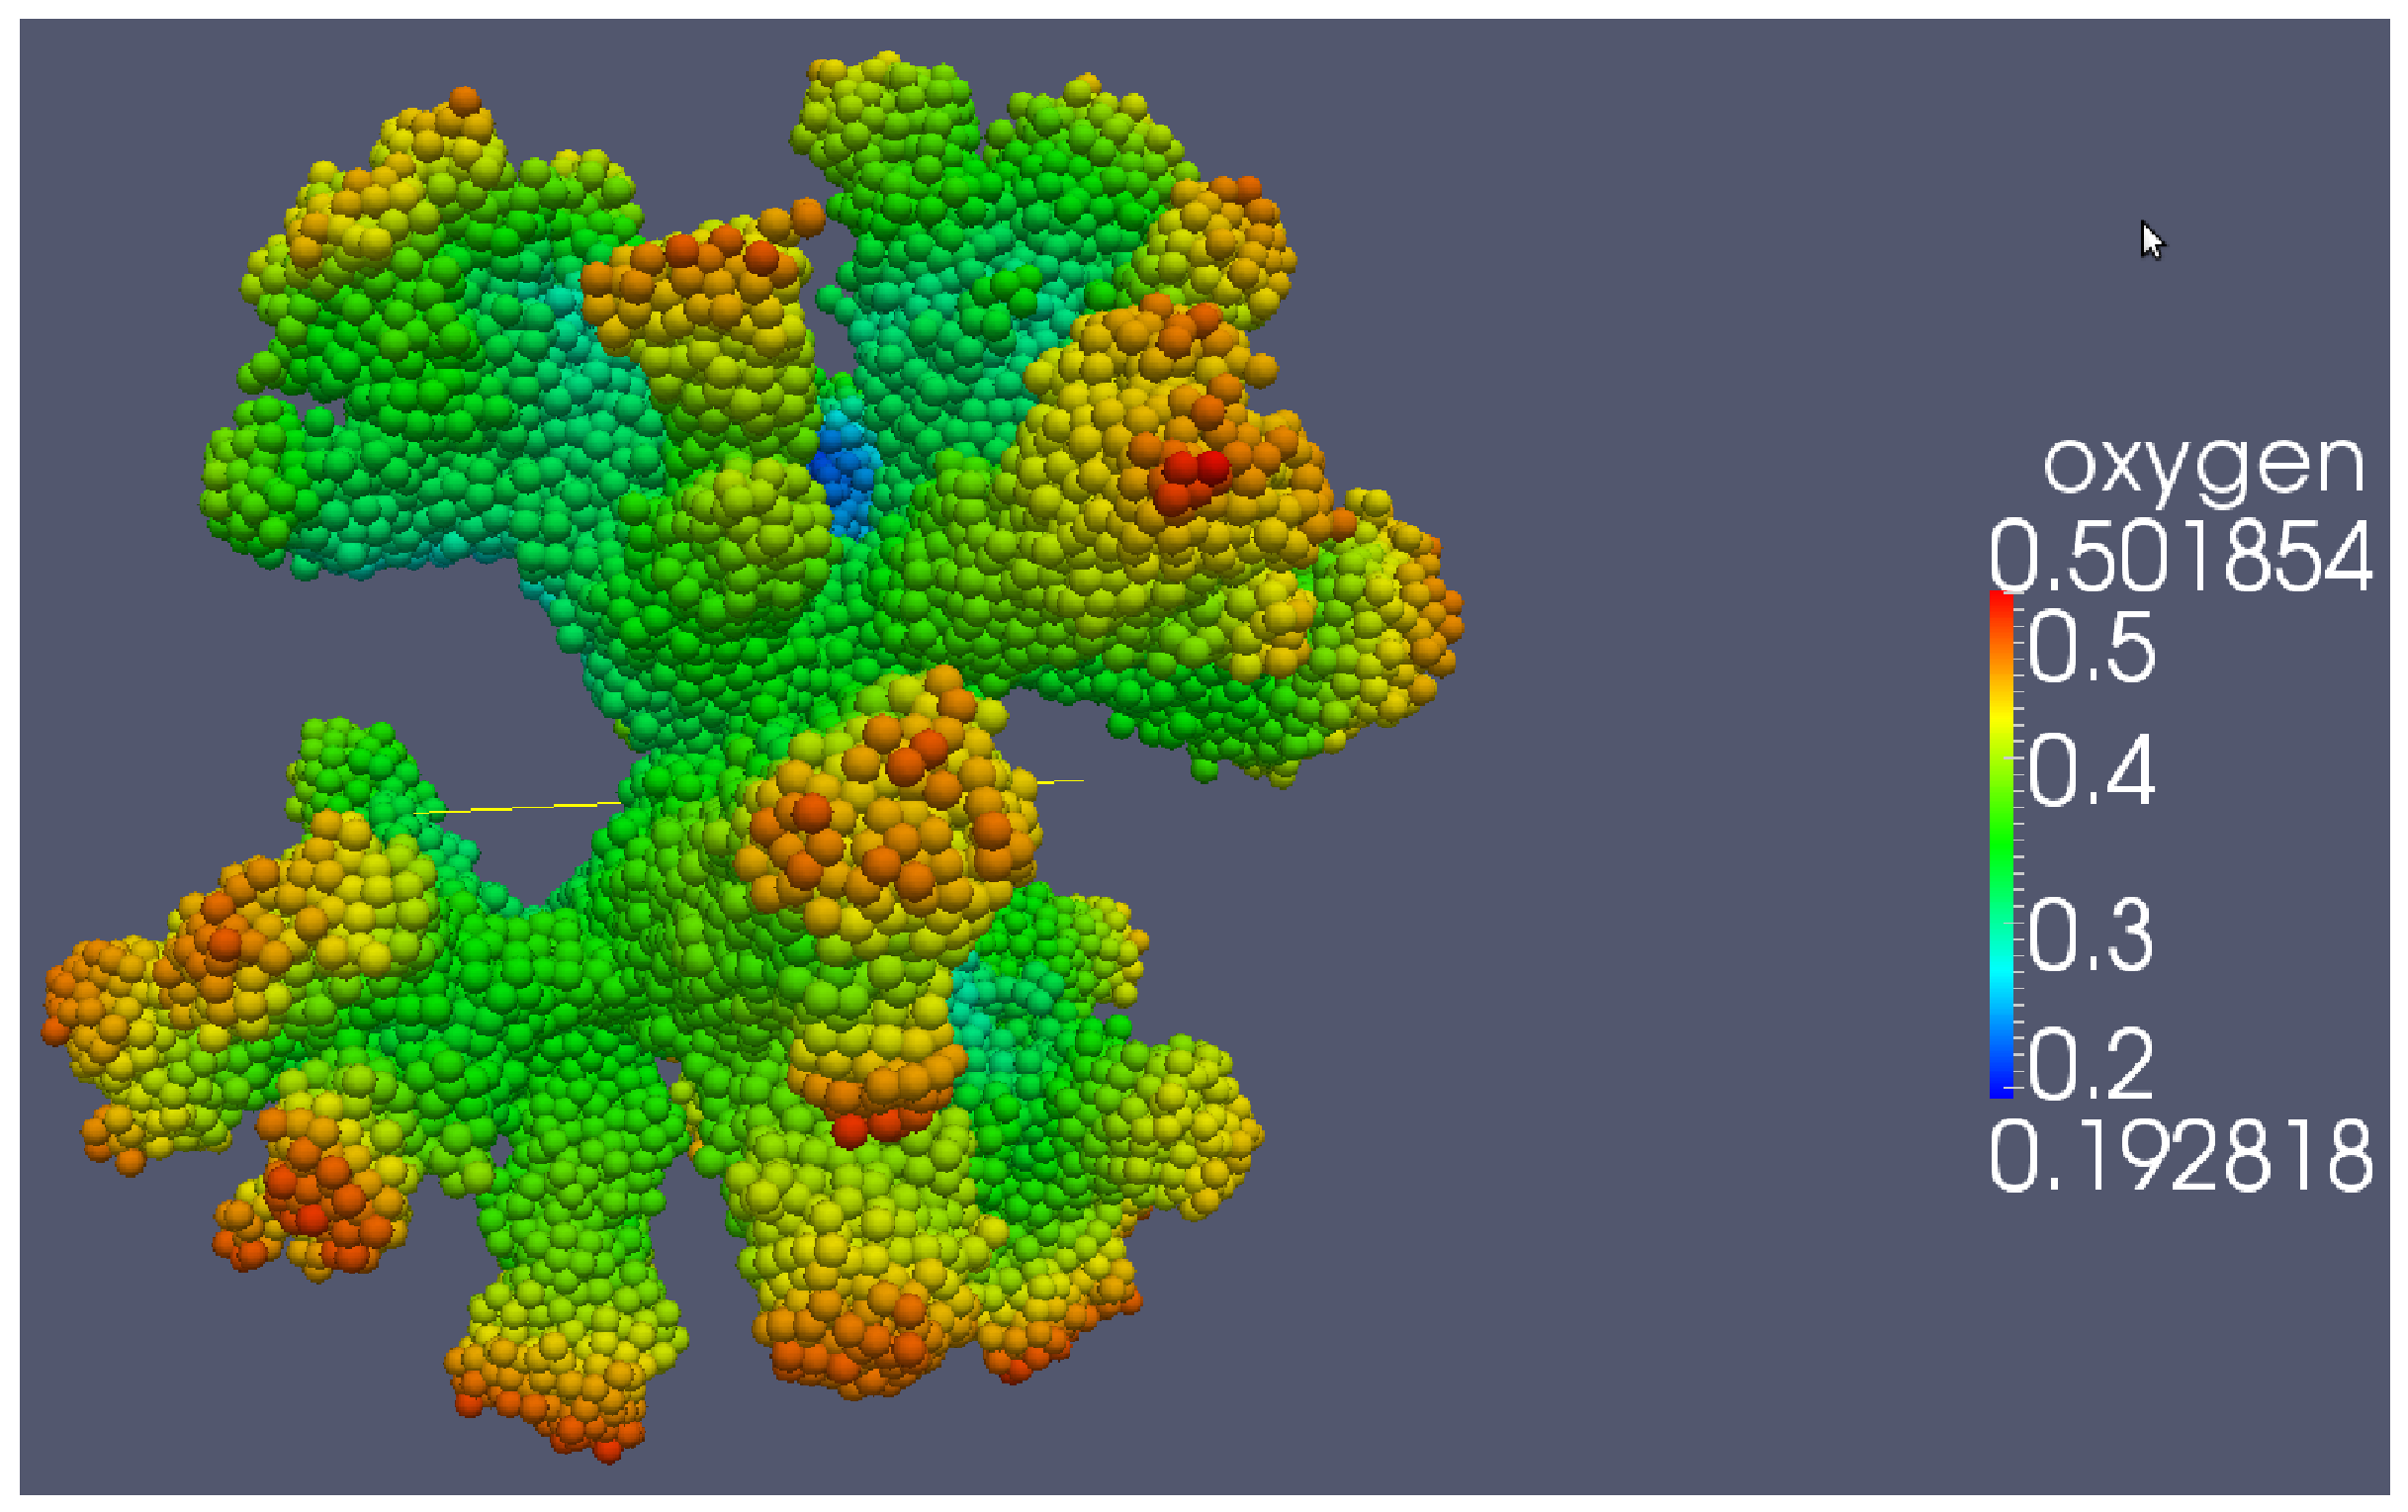
\includegraphics[width=0.8\linewidth]{images/spheroid.eps}
\end{center}
\caption{
{\bf 3D off-lattice simulation coupled to PDE: A 3D tumour spheroid with growth and death dependent on diffusion and uptake of oxygen}.
\highlight{Er - can we make this a 3D cross section that looks like Alex's old 2D sim?}
The code for this is available to download as supplementary material and can also be found at \texttt{http://chaste.here}.
}
\label{fig:TumourSpheroid}
\end{figure}

\begin{figure}[!htbp]
\begin{center}
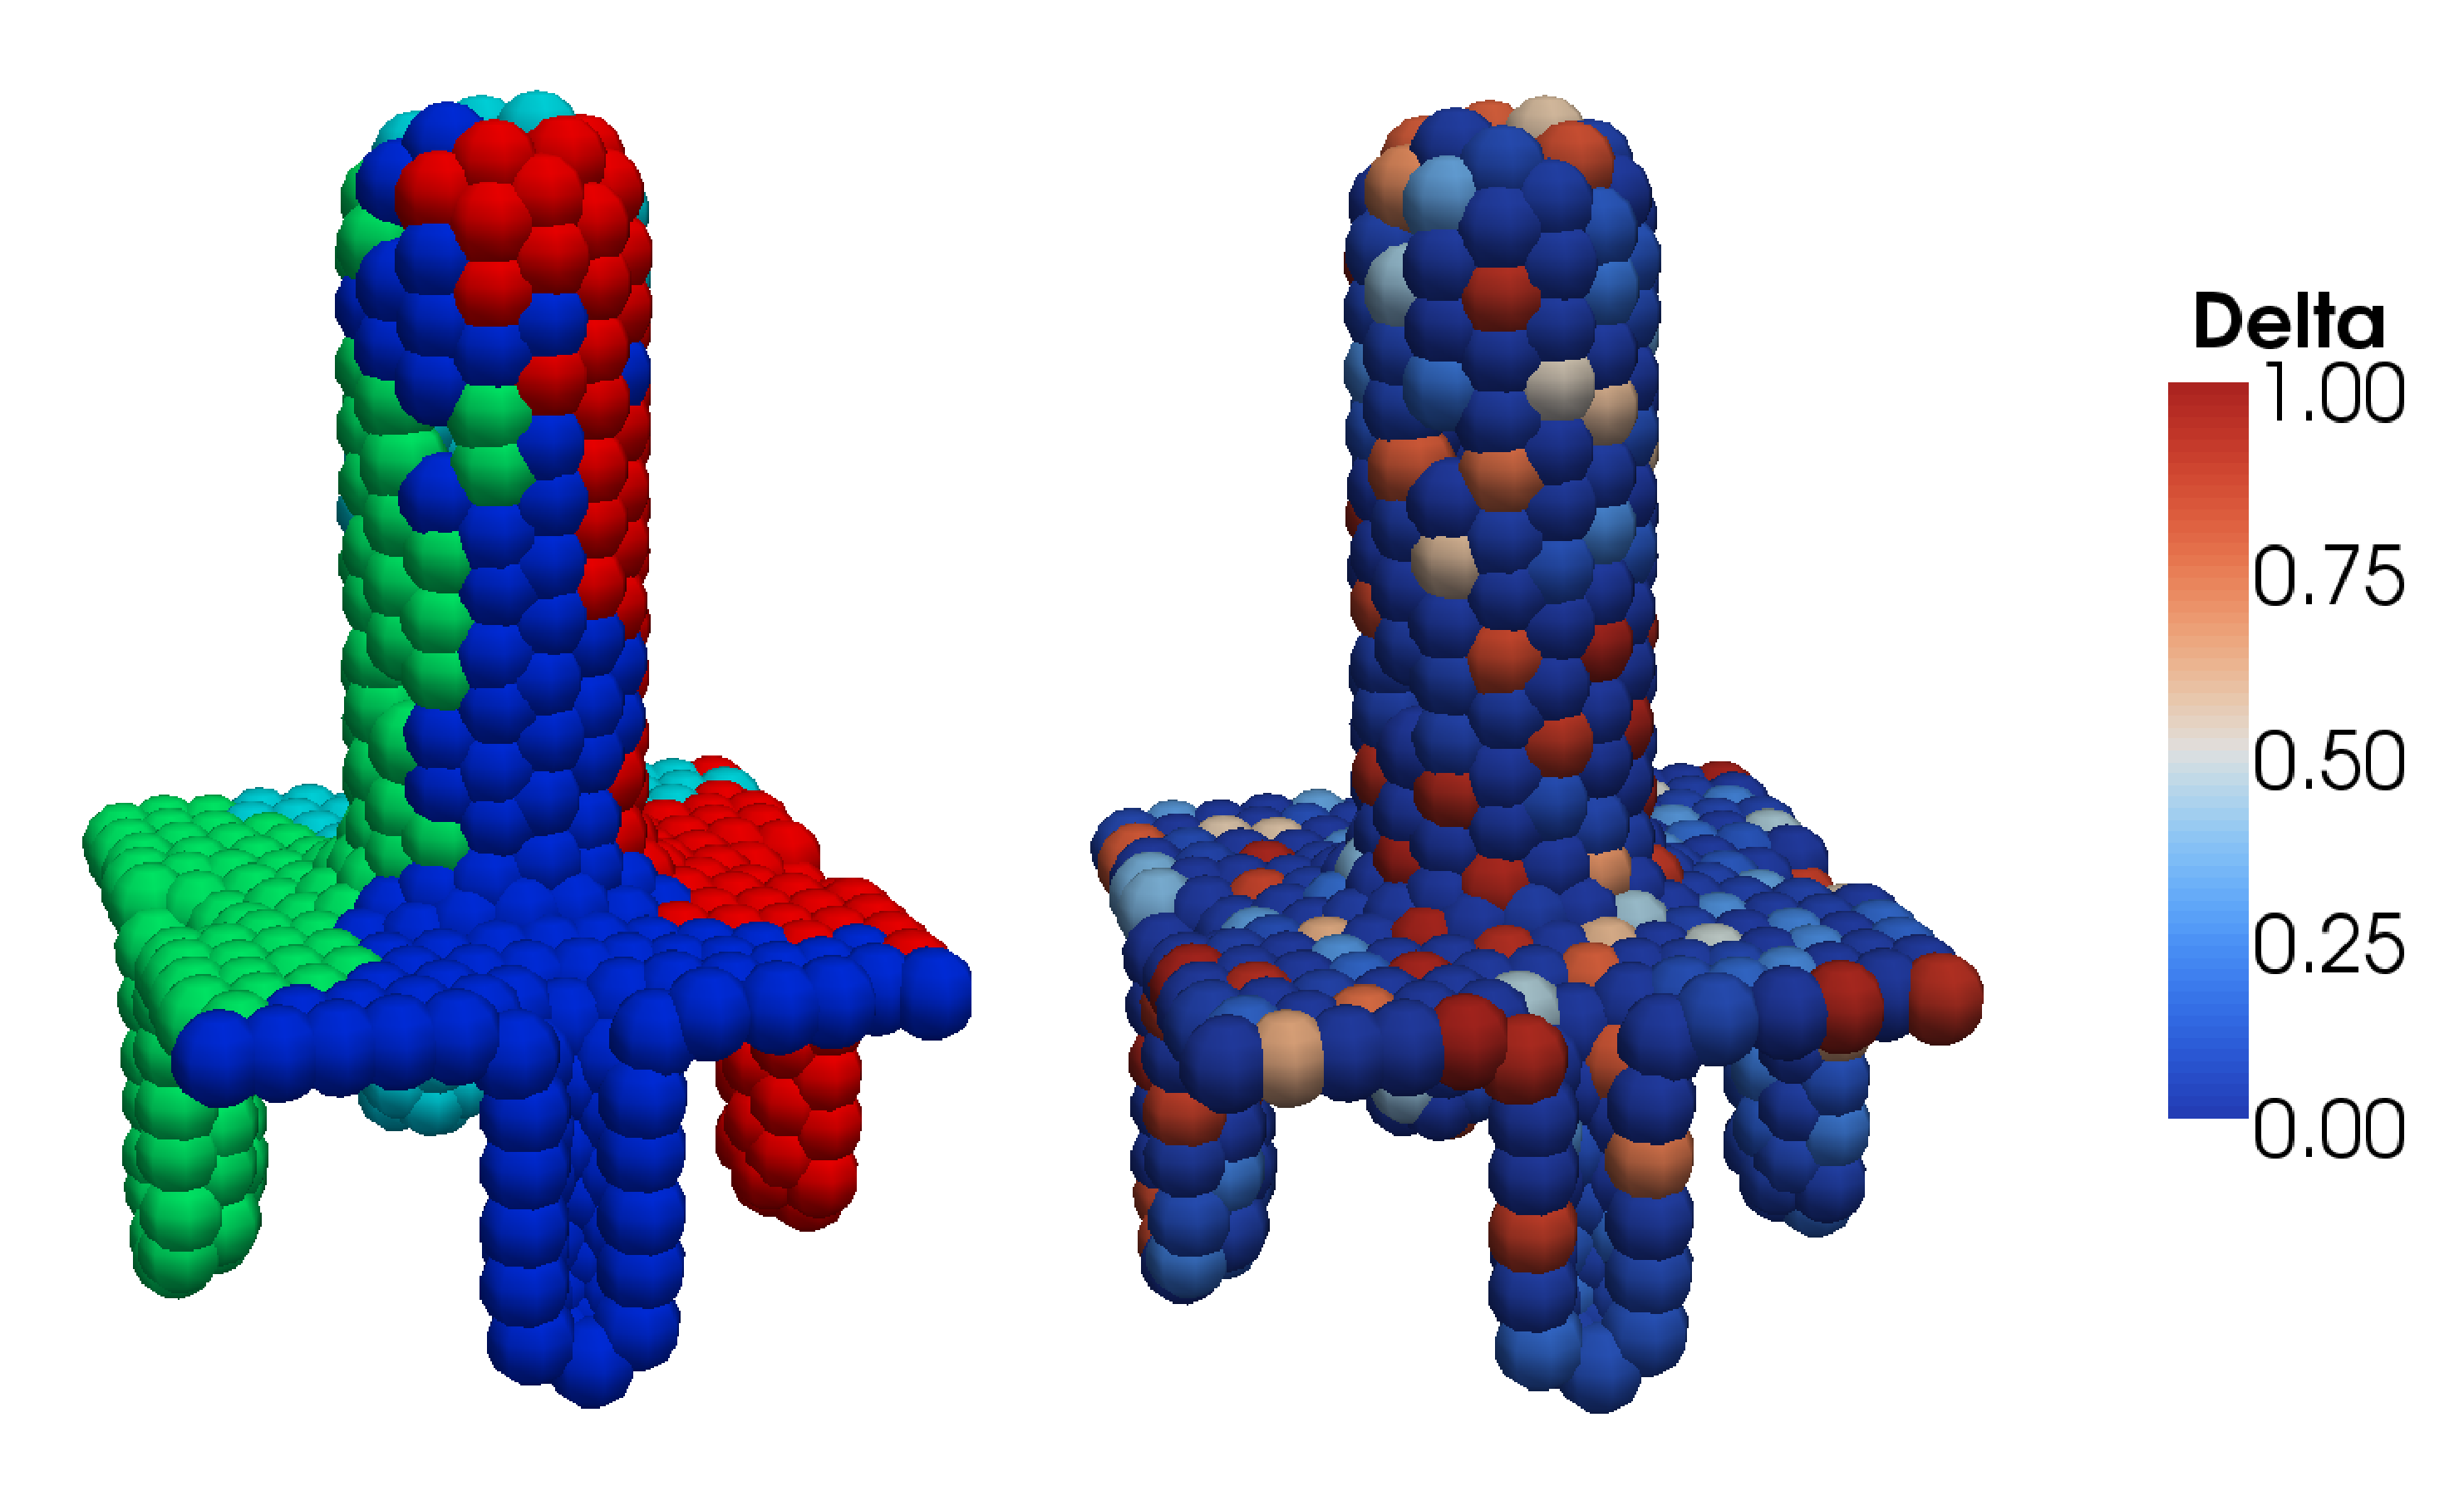
\includegraphics[width=0.5\linewidth]{images/multi_crypt.eps}
\end{center}
\caption{
{\bf 3D off-lattice simulation on a 2D surface: small intestinal crypts and villus}.  
The code for this is available to download as supplementary material and can also be found at \texttt{http://chaste.here}. 
\highlight{Possibly combine the delta-notch from Buske with this 4 crypts and a villus simulation? 
Would get nice pattern of secretory / absorptive cells presumably, which they reckon is delta-notch $\approx$ SCIENCE!
So one figure like the above with lineage tracing, and one with delta/notch patterning.}
}
\label{fig:FourCrypts}
\end{figure}

\begin{figure}[!htbp]
\begin{center}
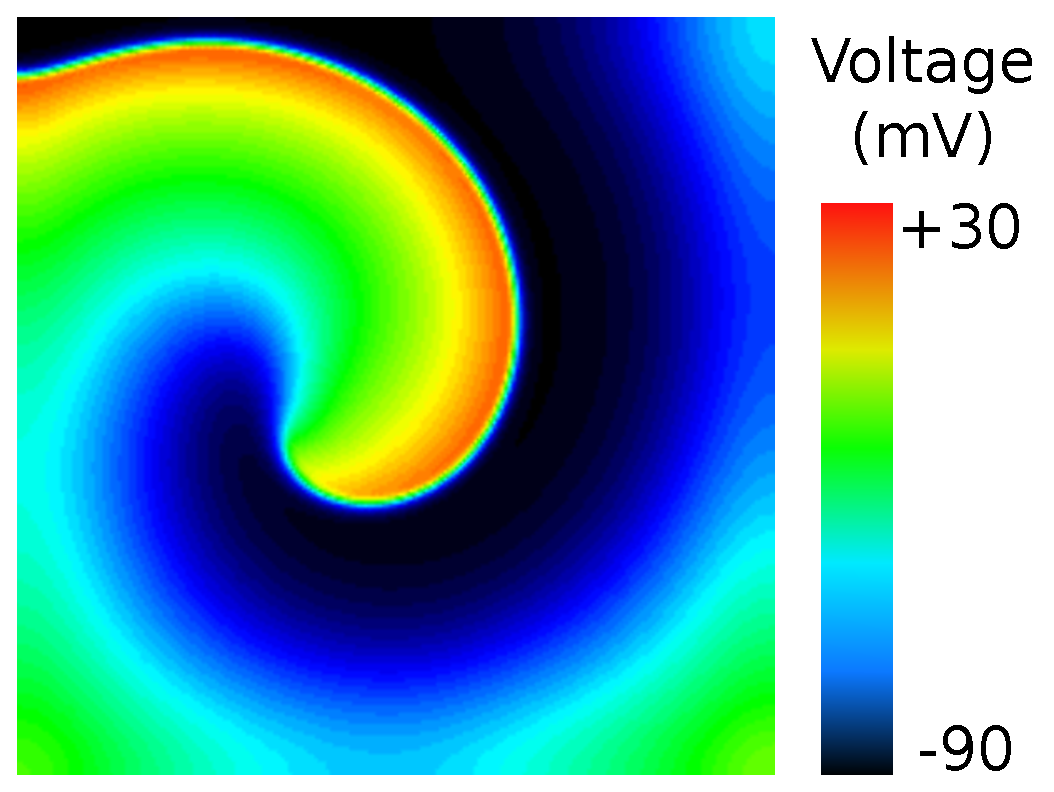
\includegraphics[width=0.5\linewidth]{images/spiral_wave.eps}
\end{center}
\caption{
{\bf Cardiac electrophysiology: a re-entrant spiral wave}.
This figure displays the membrane voltage in a 2D 3cm x 3cm using the Luo-Rudy 1991 model \cite{luo1991model} with the modifications and protocol suggested in \cite{qu2000origins}.
The code for this is available to download as supplementary material and can also be found at \texttt{http://chaste.here}.
}
\label{fig:SpiralWave}
\end{figure}

\begin{figure}[!htbp]
\begin{center}
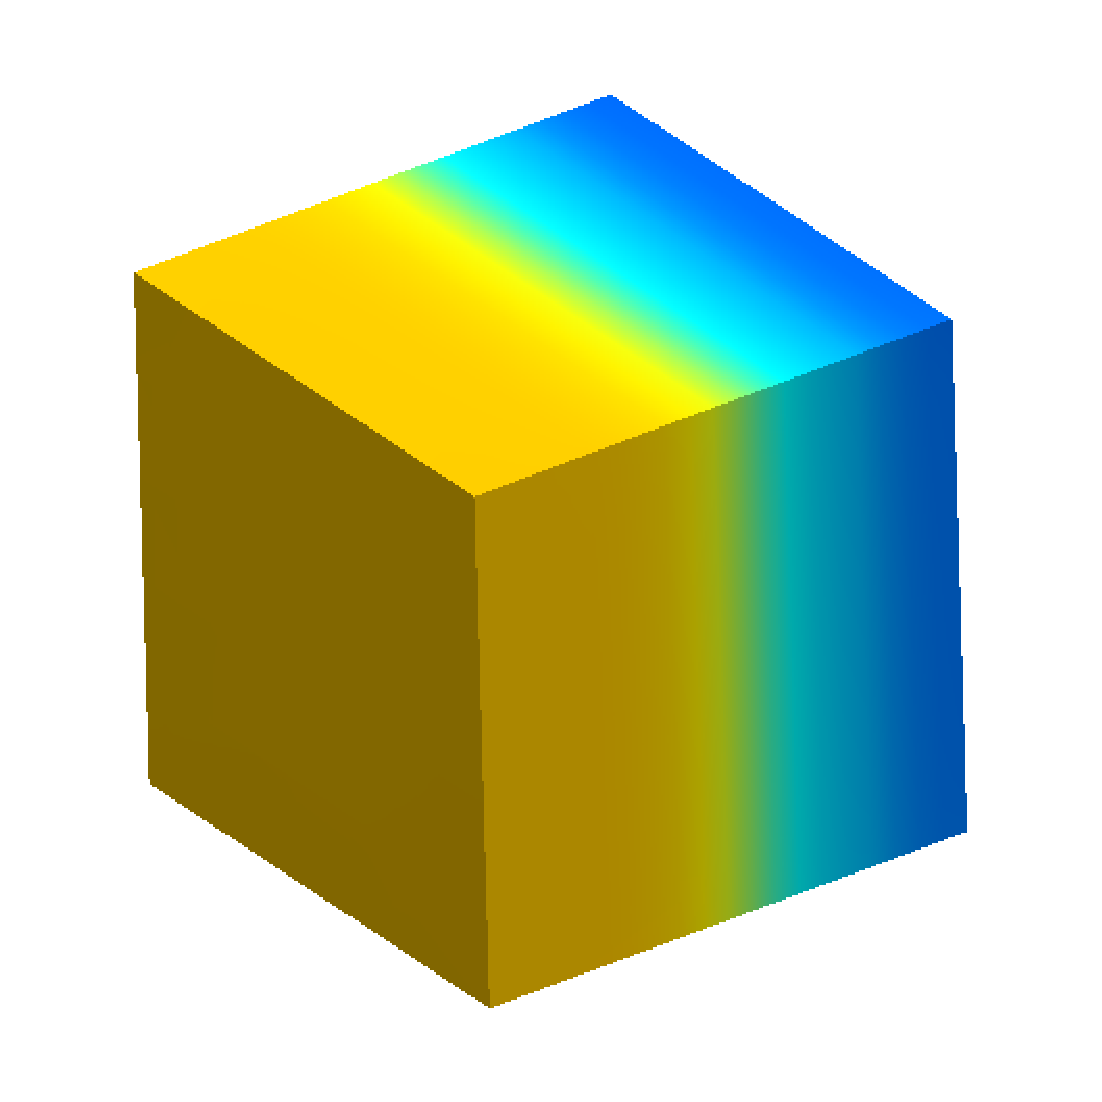
\includegraphics[width=0.4\linewidth]{images/undeformed_cube.eps}
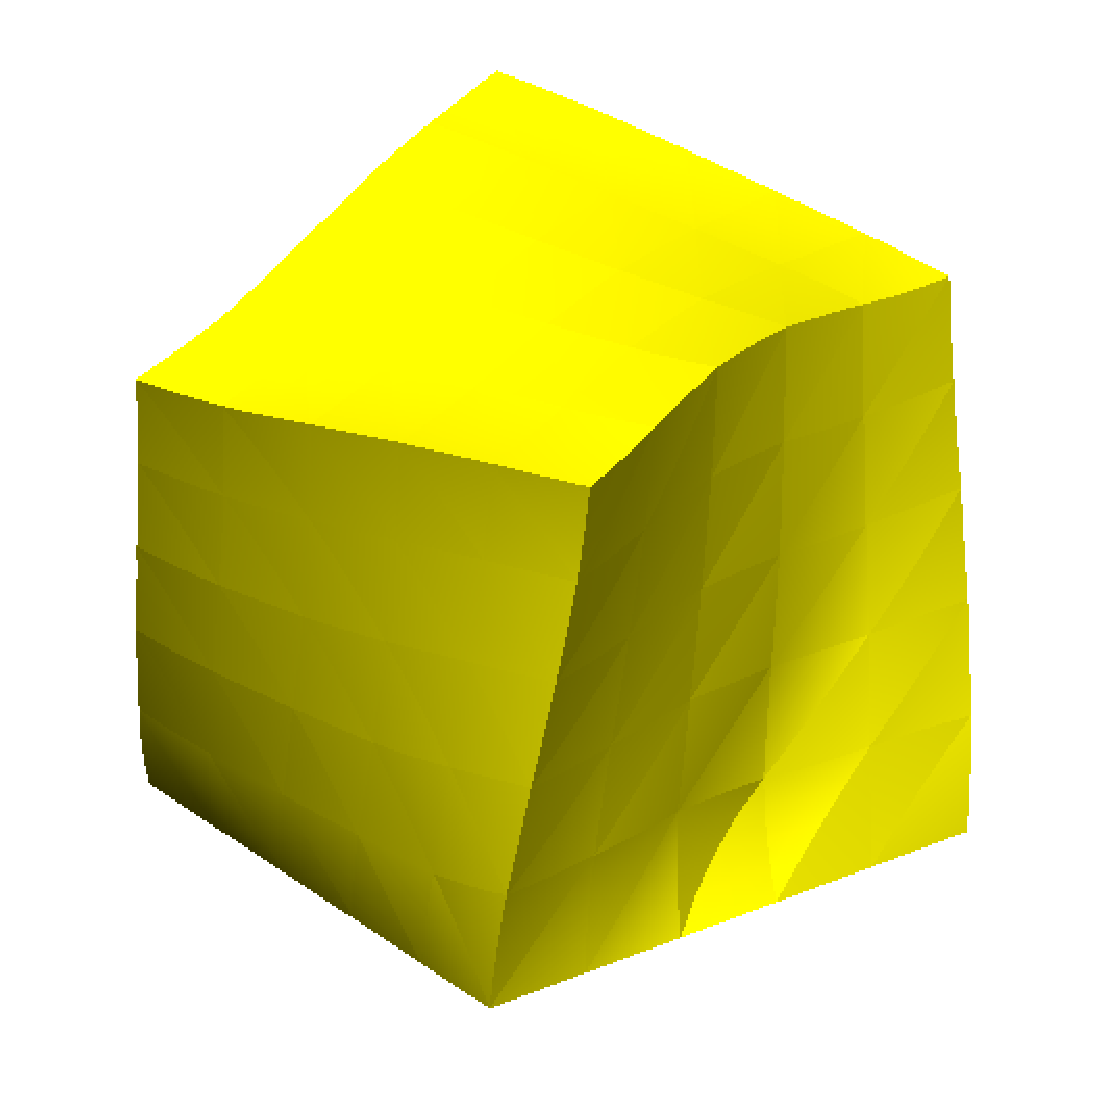
\includegraphics[width=0.4\linewidth]{images/deformed_cube.eps}
\end{center}
\caption{
{\bf Cardiac electromechanics: simulation of electrical propogation and subsequent deformation in a ventricular wedge with non-uniform fibre orientation}.  
The code for this is available to download as supplementary material and can also be found at \texttt{http://chaste.here}.
\highlight{Can we have three figures - fibre directions, electrical wave propogation at about half way (still mostly undeformed), and a fully deformed (depolarized) cube?}\comment{PP: put electrical activity in these figures and make them colour}
}
\label{fig:TwistyWedge}
\end{figure}

%%%%%%%%%%%%%%%%%%%%%%%%%%%%%%%%%%%%%%%%%%%%%%%%%%%%%%%%%%%
%%%% Any tables in the document go here.
%%%%%%%%%%%%%%%%%%%%%%%%%%%%%%%%%%%%%%%%%%%%%%%%%%%%%%%%%%%
%\section*{Tables}

%%%%%%%%%%%%%%%%%%%%%%%%%%%%%%%%%%%%%%%%%%%%%%%%%%%%%%%%%%%
%%%% THIS WILL BE ONLINE - NOT TO BE INCLUDED IN WORD COUNT
%%%%%%%%%%%%%%%%%%%%%%%%%%%%%%%%%%%%%%%%%%%%%%%%%%%%%%%%%%%

\newpage
\section*{Supplementary Material}

\section{Installation}

In this section we summarise how to install and run Chaste.
The simplest method is to use the Ubuntu Linux operating system, as a package is available for this platform.
Instructions for this are at:\\
\texttt{https://chaste.cs.ox.ac.uk/cgi-bin/trac.cgi/wiki/InstallGuides/UbuntuPackage}.
In practice many users find it easiest to install Chaste on a virtual machine running Ubuntu, if no Ubuntu machine is available.

Chaste can also be installed on any other Linux system. 
Manual installation of a number of dependencies is required, but scripts are provided to simplify this process.
Instructions are here:\\
\texttt{https://chaste.cs.ox.ac.uk/cgi-bin/trac.cgi/wiki/InstallGuides}

The bolt-on project \texttt{Plos2012} is available to download from \highlight{finish}

\section{Dependencies}

\begin{table}[!ht]
    \caption{
    \bf{Chaste Dependencies.} For the full text of all licences examine the contents of \texttt{docs/licences.html} 
    or visit \texttt{https://chaste.cs.ox.ac.uk/cgi-bin/trac.cgi/export/14566/trunk/docs/Licences.html}
    \comment{JC: Update to a release version.}}
    \begin{tabular}{|l|l|l|}
      \hline
      Dependency & Available from & Licence \\
\hline
Amara & \texttt{http://wiki.xml3k.org/Amara} & Apache 1.1\\
Boost & \texttt{http://www.boost.org} & Custom\\
CodeSynthesis XSD &  \texttt{http://codesynthesis.com/products/xsd} & GPL\\
CVODE (SUNDIALS) & \texttt{https://computation.llnl.gov/casc/sundials} & BSD\\
CxxTest & \texttt{http://cxxtest.tigris.org} & LGPL\\
HDF5 &  \texttt{http://www.hdfgroup.org/HDF5/HDF5.txt} & Custom\\
(Par)METIS &  \texttt{http://glaros.dtc.umn.edu/gkhome/views/metis} & Custom\\
MPICH &  \texttt{http://www.mcs.anl.gov/research/projects/mpich2} & Custom\\
PETSc &  \texttt{http://www.mcs.anl.gov/petsc} & Custom\\
Pyparsing &  \texttt{http://pyparsing.wikispaces.com} & MIT\\
RDFLib &  \texttt{https://github.com/RDFLib} & BSD\\
RNV &  \texttt{http://www.davidashen.net/rnv.html} & BSD\\
TetGen &  packaged with Chaste & Custom\\
triangle &  packaged with Chaste & Custom\\
VTK &  \texttt{http://www.vtk.org} & BSD\\
Xerces &  \texttt{http://xerces.apache.org/xerces-c} & Apache 2 \\
      \hline
    \end{tabular}
    \begin{flushleft}
    \end{flushleft}
    \label{tab:ChasteDependencies}
\end{table}

\end{document}

